\foreach \metric/\cap in \metrics{
    \begin{figure}[h!]
        \centering
        \includegraphics[width=\textwidth]{chapters/experiments/img/merged_plots/per1_all/\metric.png}
        \caption{\cap \space w zależności od liczby wierzchołków}
        \label{fig:small_\metric}
    \end{figure}
}

\begin{figure}[h!]
    \centering
    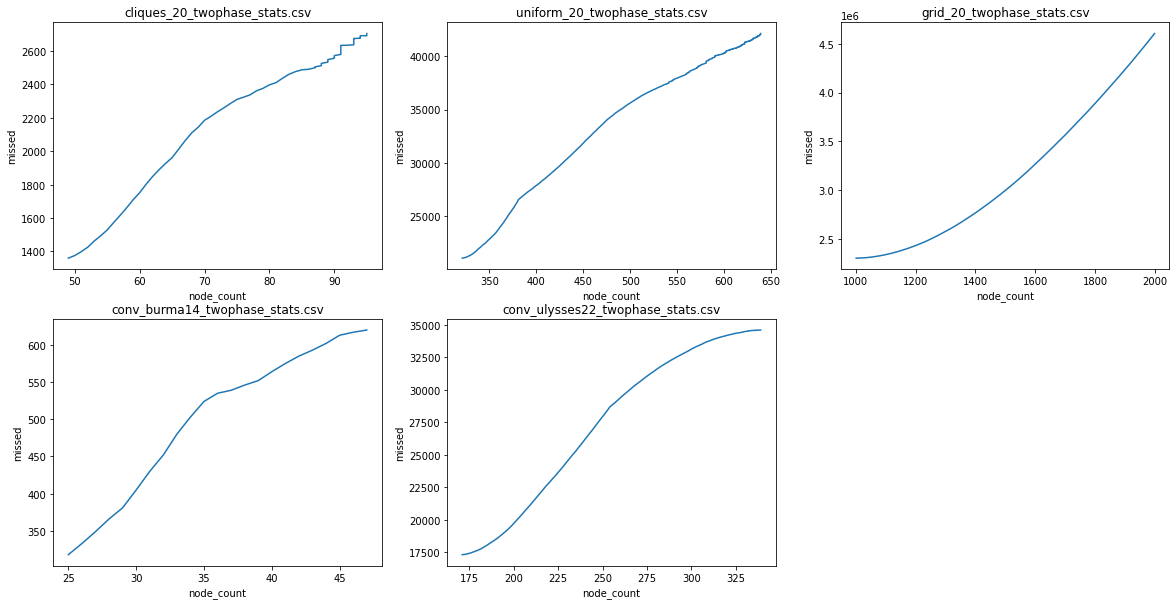
\includegraphics[width=\textwidth]{chapters/experiments/img/merged_plots/per1_all/missed.png}
    \caption{Liczba nieudanych prób tworzenia krawędzi w zależności od liczby wierzchołków --- próbkowanie dwufazowe}
    \label{fig:small_missed}
\end{figure}
